\subsection{Normal Enhancement Operators}
The paper \cite{referencePaper} describes two types of normal variations: \textit{smoothing} and \textit{sharpening}. Those two kind of enhancement operators works on the high-frequency components of the surface normal. Smoothing reduces those components, while Sharpening increase them. 
\subsubsection{Normal Smoothing Operator Implementation}
To calculate smoothed surface normal I started from this idea\footnote{\url{https://www.reddit.com/r/opengl/comments/6976lc/smoothing_function_for_normals/}}. The implementation of normal smoothing operator was done in model\char`_v1 file, while \textit{processing the Assimp mesh} in order to obtain an \textit{OpenGL mesh}. I created a \textbf{new position in the vertex attribute}, that stores smoothed normal. \newline
In this way, data can be loaded in vertex shader by simply add the line in \textbf{Code \ref{code:vert_smoothing}}. \newline
The smoothing normal computation is done for each vertex. I \textbf{initialized} it to vector zero. Then, I \textbf{computed face normal} for each face of the mesh and I \textit{added} it to each vertex of the face. Finally, for each vertex, I \textbf{normalized the result} of this sum. \newline
By doing so, I implicitely consider the \textit{kernel} of convolution as the \textit{smallest one}, considering as \textbf{neighbourhood} only the faces that share the same vertex. I also implicitely defined the \textit{$\sigma$} parameter, found in Equation 5 of 4.2.1 chapter of \cite{referencePaper} that \textit{weights} this operation as \textit{1}. This greatly \textbf{simplifies} computation and code while maintaning the same \textit{intent} as the original paper. The added lines of code are showed in \textbf{Code \ref{code:smoothing_model}}.
\begin{lstlisting}[language=C++, caption=Smoothed normal loaded in vertex shader,label={code:vert_smoothing}]
layout (location = 2) in vec3 sm_normal;	
\end{lstlisting}
\begin{lstlisting}[language=C++, caption=Smoothed normal computations added in processMesh method of model\char`_v1 file ,label={code:smoothing_model}]
	for(GLuint i = 0; i < mesh->mNumVertices; i++)
	{
		Vertex vertex;
		...
		vertex.Sm_Normal = glm::vec3();
		...
	}
	// For each face, I calculate the face normal and I add to the vertices' normal used by the face. Finally, I normalize the normal to obtain the smoothed surface normal.
	for ( int i = 0; i < indices.size(); i += 3 )
	{
		// I Compute the face normal using triangleNormal method, that computes normal starting from triangle points
		glm::vec3 faceNormal = glm::triangleNormal(
		vertices[indices[i]].Position,
		vertices[indices[i+1]].Position,
		vertices[indices[i+2]].Position);
		
		
		
		// I add face normal to each of the 3 vertex normal of the face
		for ( int j = 0; j < 3; j++ )
		{
			vertices[indices[i+j]].Sm_Normal += faceNormal;
		}
	}
	for (auto &v : vertices)
	{
		// Normalizing the vectors accumulating face normals to obtain the smoothed surface normal
		// NOTE: Sigma parameter, found in Equation 5 of 4.2.1 chapter of the reference paper ( to control the quantity of convolution kernel used ) is implicitely 1.
		v.Sm_Normal = glm::normalize(v.Sm_Normal);
	}	
\end{lstlisting}
\subsubsection{Normal Sharpening Operator Implementation}
Normal Sharpening operator is implemented in \textbf{fragment shader} and uses the smoothed normal previously described and passed to the \textit{vertex shader}. \newline
In vertex shader, I apply \textit{normal Matrix transformation} before passing them to the fragment shader as showed in \textbf{Code \ref{code:vert_sharpening}} . \newline
In fragment shader, I calculate the \textbf{mask} by subtracting the original normal vector with its smoothed version. Then, I add the mask multiplied by a \textbf{scaling factor} $\lambda$ to the normal vector, with a typical process called \textbf{unsharp masking} as described in Equation 6 of 4.2.2 chapter of \cite{referencePaper}. Finally, I normalize the result. \newline
The \textbf{Code \ref{code:frag_sharpening}} is added to the fragment shader to implement this process.
\begin{lstlisting}[language=C++, caption=Transformation applied to smoothed normal in vertex shader,label={code:vert_sharpening}]
	vSMNormal = normalize( normalMatrix * sm_normal );
\end{lstlisting}
\begin{lstlisting}[language=C++, caption=Calculation of normal sharpening operator in fragment shader,label={code:frag_sharpening}]
	// Computing the mask for Unsharp Masking
	vec3 mask = vNormal - vSMNormal;
	// calculating enhanced Normal using the Unsharp Masking technique. This is defined, in the reference paper, in equation 6 of chapter 4.2.2
	vec3 eNormal = vNormal + lambda * mask;
	// normalization of the per-fragment enhanced normal 
	vec3 N_I = normalize(eNormal);	
\end{lstlisting}
A Comparison between normal vector and enhanced normal vector (through sharpening) is showed in \textbf{Figure \ref{fig:normal_comparison}} that shows two subroutines created in the project.
\pagebreak
\begin{figure}[h]
	\centering
	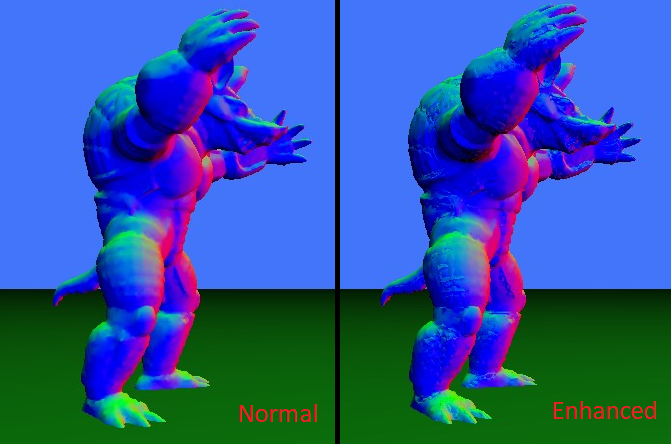
\includegraphics[width=0.8\textwidth]{Images/normal_comparison.png}
	\caption{Comparison between normal and enhanced normal vector (through sharpening)}
	\label{fig:normal_comparison}
\end{figure}